\documentclass[12pt]{article}

\usepackage{amsmath}
\usepackage{amssymb}
\usepackage{bm}
\usepackage{minted}
\usepackage{enumerate}
\usepackage{fancyvrb}
\usepackage[top=1in, bottom=1in, left=1in, right=1in]{geometry}
\usepackage{hyperref}
\usepackage{placeins}
\usepackage{tikz}
\usepackage{tikzsymbols}
\usepackage[most]{tcolorbox}
\usepackage{enumitem}
\usepackage{algpseudocode,algorithm,algorithmicx}
\newcommand*\DNA{\textsc{dna}}
\usetikzlibrary{positioning,calc}
\usepackage{graphicx}
\usepackage{amsmath}
%-------------------------------------------------------------------------------
% Custom commands
\usepackage{xcolor} %hilight
\newcommand{\hilight}[1]{\colorbox{yellow}{#1}}
%-------------------------------------------------------------------------------

\newtcolorbox[]{solution}[1][]{%
    breakable,
    enhanced,
    colback=white,
    title=Solution,
    #1
}


\begin{document}
\begin{center}
  \centerline{\textsc{\LARGE  Homework 1}}
  \vspace{1em}
  \textsc{\large CMU 16-782 : Planning and Decision Making in Robotics} \\
\end{center}

\section*{Implementation details}
\begin{enumerate}
    \item I have implemented a simple Dijkstra planner for this homework. The planner starts from the current position of the robot and calculates the optimum g as well as the path steps to every node in the map. After this, I calculate the target node where my robot need to go and backtrack to calculate the path. All of this is done in the first time step only.   
    \item After the g value and the path time to every node in the map is calculated, the algorithm loops over every point in the target trajectory and picks up the point where the total cost of reaching plus waiting is minimized.
    
    \item I have used a priority queue(open\_list) of pointers to the nodes for my open list, an unordered map(openPtrList) for maintaining the pointers to all the nodes which have been visited(the key in this unordered map is obtained from GETMAPINDEX), an unordered map(closedPtrList) to maintain if I have expanded a node or not(the key in this unordered map is obtained from GETMAPINDEX).
    
    \item \textbf{Open list} : The data structure I have used for maintaining my open\_list is a priority\_queue. I maintain a priority queue of pointers to the nodes, arranged according to their decreasing g-value. Since we can not access any pointer in a priority queue, after popping a pointer off the open list, I check if it has been closed or not. The node is expanded only if it has not been expanded before. \\
    Open list is open\_list in my code. 
    
    \item \textbf{Closed list} : I have used an unordered map for maintaining my closed list. This unordered map uses the GETMAPINDEX as it's key and a boolean as it's value. \\
    Closed list is closedPtrList in my code.
    
    \item \textbf{Open pointer list} : I have used an unordered map for maintaining a directory of pointer to the nodes which have been visited before. This is important so that we can retrieve the pointer to nodes which have been visited. This unordered map uses GETMAPINDEX as it's key with pointer to a node as it's value.\\
    Open pointer list is openPtrList in my code.
    
    \item \textbf{Actions} : Since the path is generated only once during the first time step, I have setup two static unordered map which use GETMAPINDEX as their key and corresponding action as their value. I have setup two unordered maps to correspond to x and y steps.\\
    Actions are actions\_x and actions\_y in my code.
\end{enumerate}

\section*{Results}
\begin{enumerate}
    \item Map 1 : 
    \begin{center}
    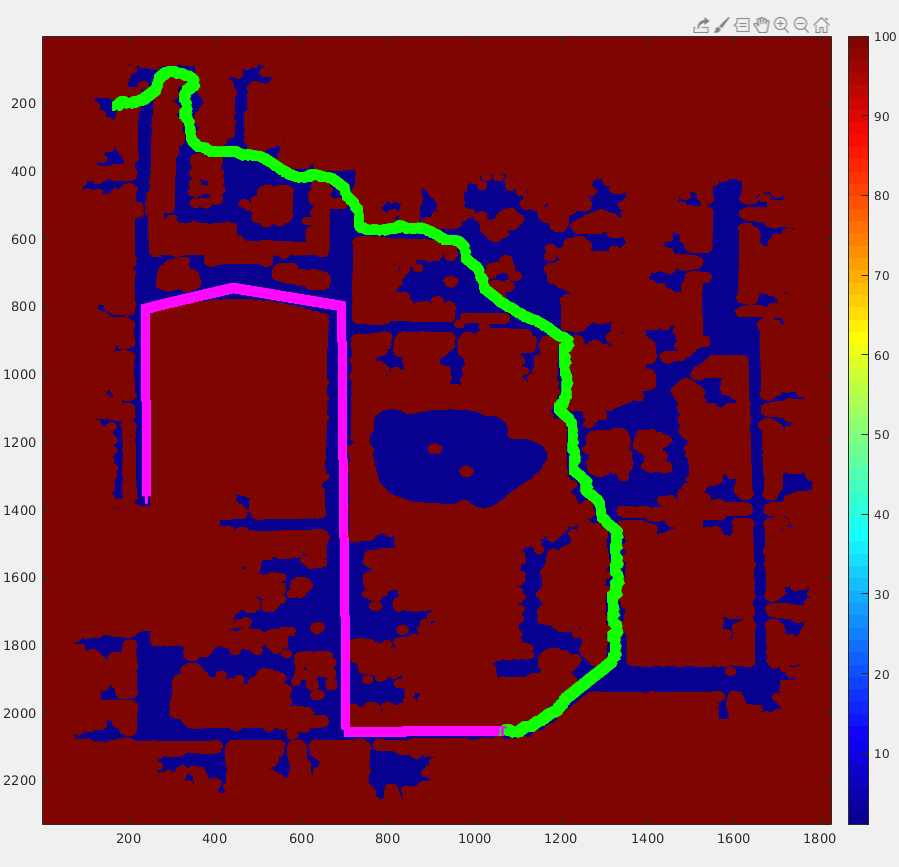
\includegraphics[scale = 0.4]{16782_HW1_fall19_v2/pictures/map1.png} \\
    \end{center}
    
    Cost Details:
    \begin{center}
    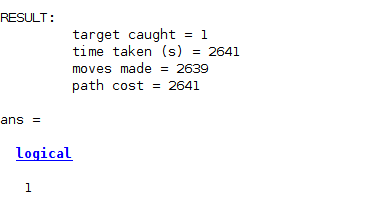
\includegraphics[scale = 0.6]{16782_HW1_fall19_v2/pictures/map1_cost.png} \\
    \end{center}
    
    \pagebreak
    
    \item Map 2 : 
    \begin{center}
    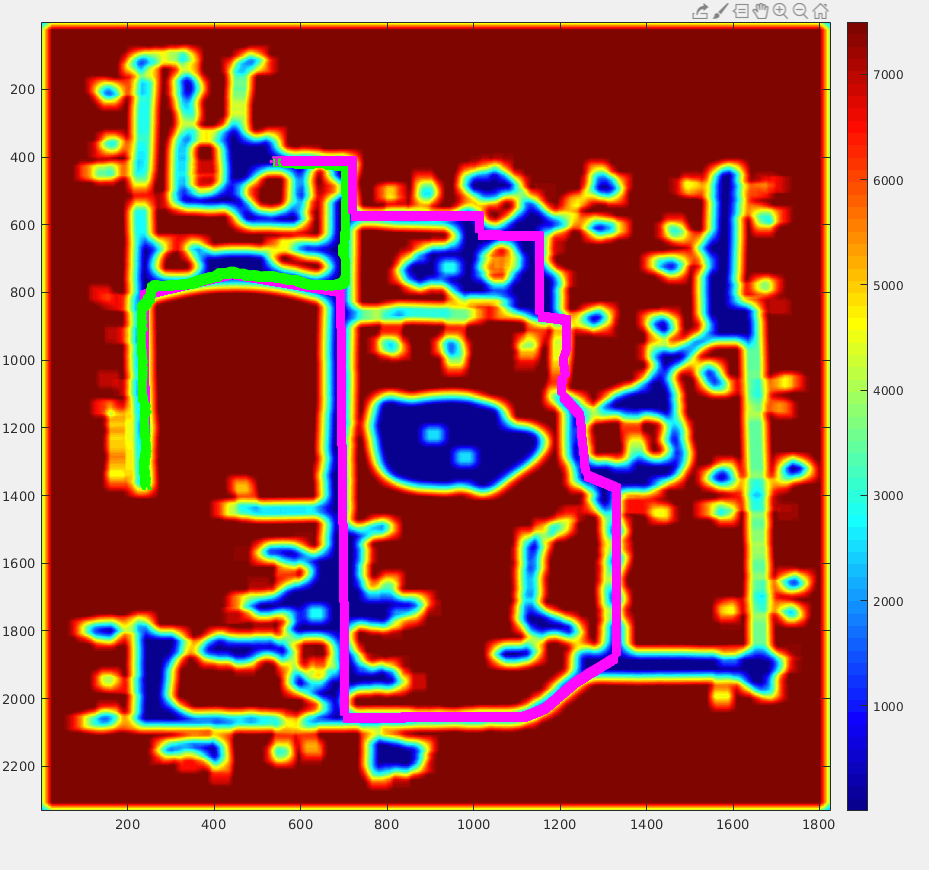
\includegraphics[scale = 0.4]{16782_HW1_fall19_v2/pictures/map2.png} \\
    \end{center}
    
    Cost Details:
    \begin{center}
    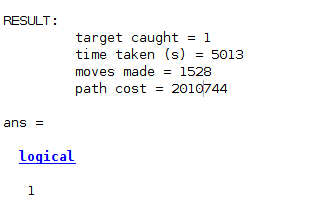
\includegraphics[scale = 0.6]{16782_HW1_fall19_v2/pictures/map2_cost.png} \\
    \end{center}
    
    \pagebreak
    
    \item Map 3 : 
    \begin{center}
    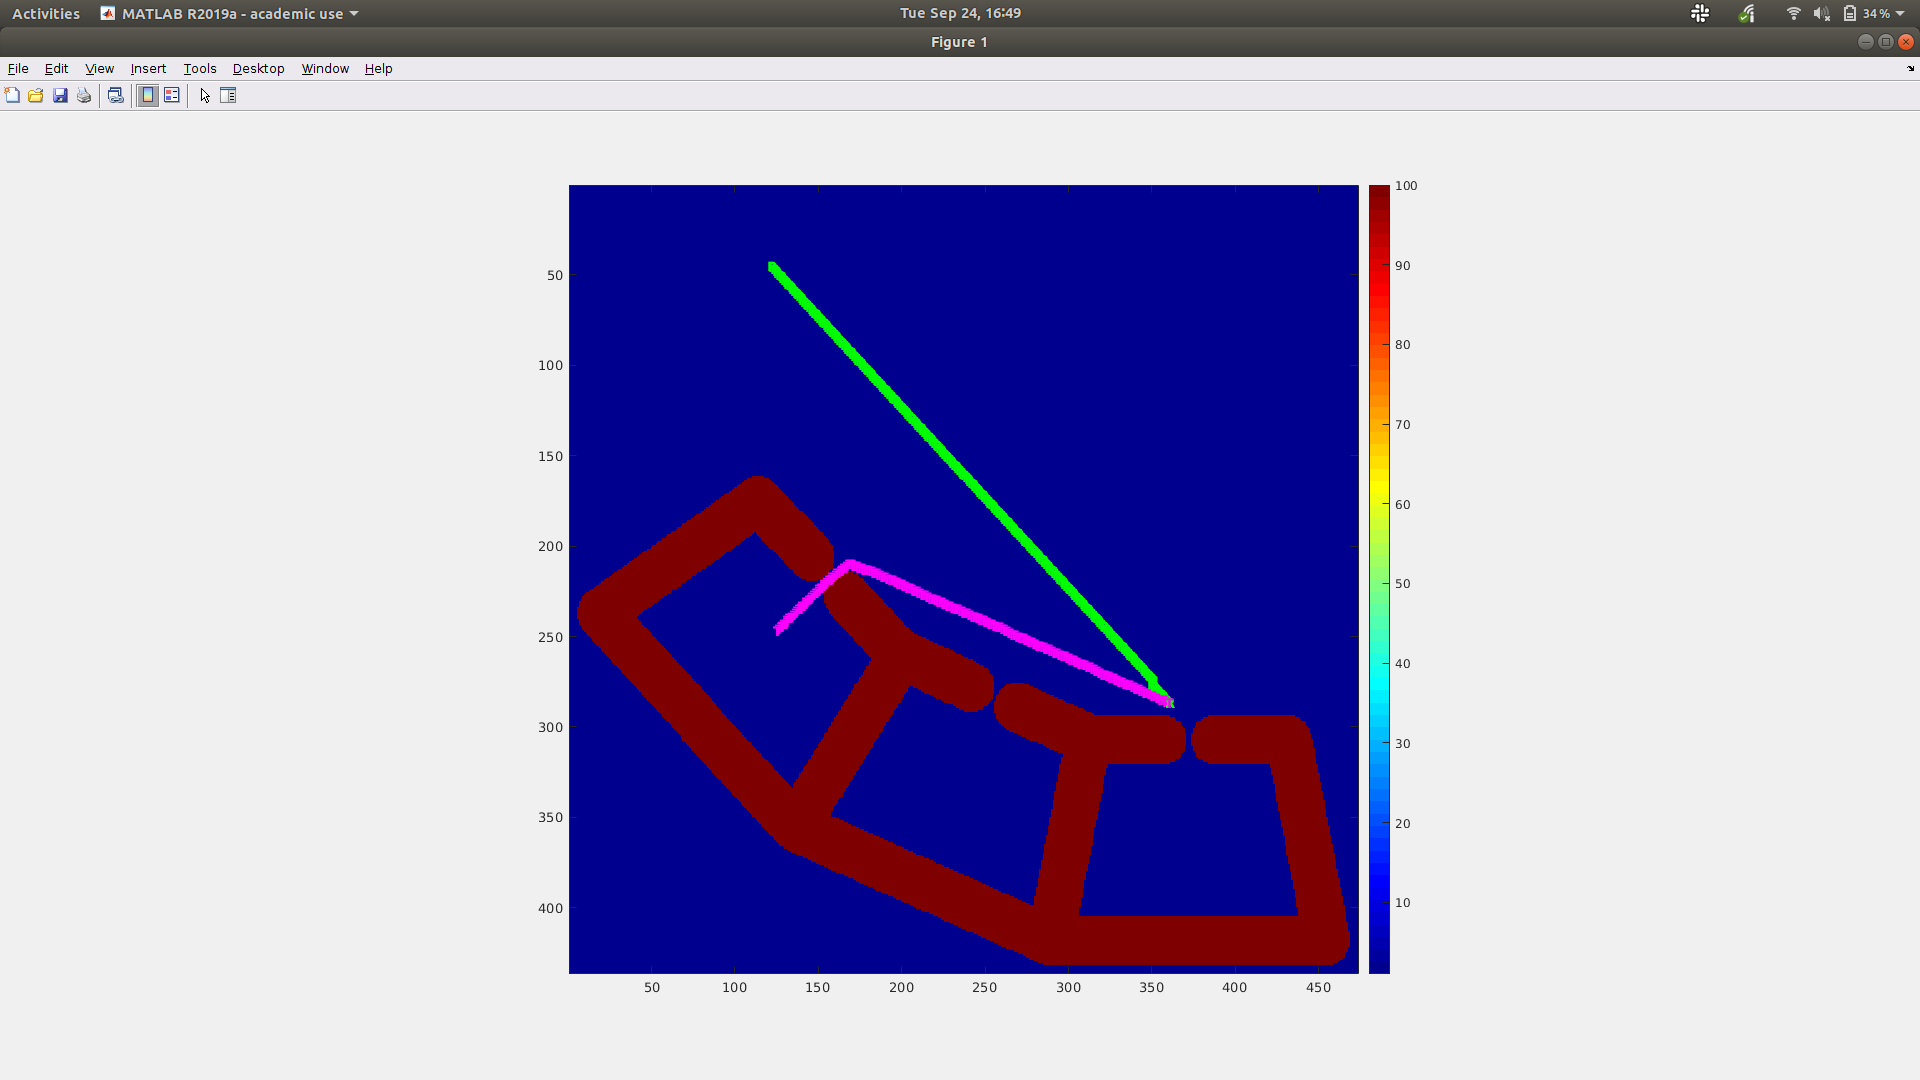
\includegraphics[scale = 0.4]{16782_HW1_fall19_v2/pictures/map3.png} \\
    \end{center}
    
    Cost Details:
    \begin{center}
    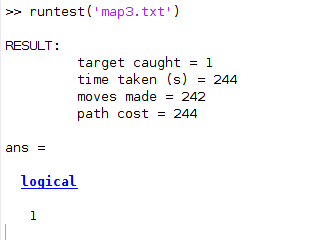
\includegraphics[scale = 0.6]{16782_HW1_fall19_v2/pictures/map3_cost.png} \\
    \end{center}
    
    \pagebreak
    
    \item Map 4 : 
    \begin{center}
    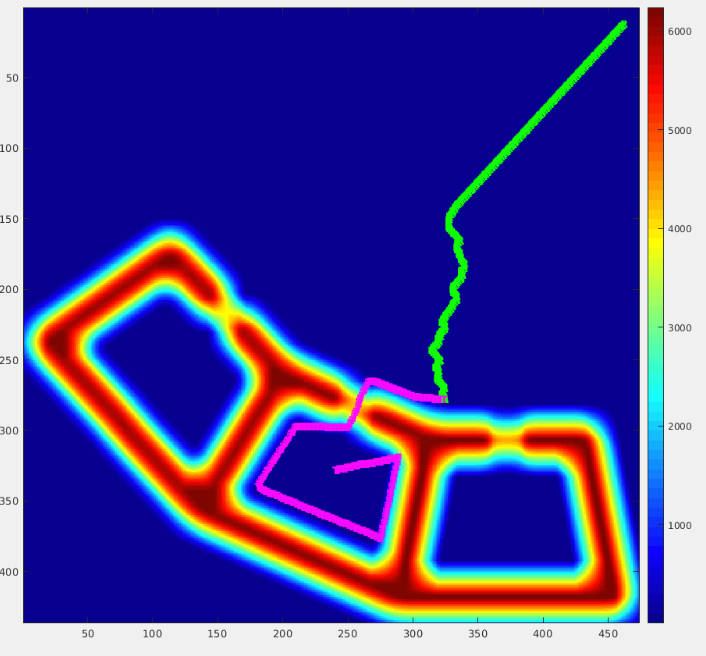
\includegraphics[scale = 0.4]{16782_HW1_fall19_v2/pictures/map4.png} \\
    \end{center}
    
    Cost Details:
    \begin{center}
    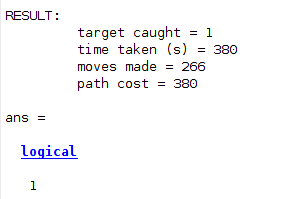
\includegraphics[scale = 0.6]{16782_HW1_fall19_v2/pictures/map4_cost.png} \\
    \end{center}
    
\end{enumerate}

\end{document}